\documentclass[12pt]{article}
\newif\ifanswer\answertrue\answerfalse% comment out to show/hide answers
\usepackage{../preamble3}% preamble always after \newif\ifanswer
%\pagenumbering{gobble}
\title{Art Of Problem Solving - AMC 10 \\ Week 8}
\author{Patrick \& James Toche}
\date{July 31, 2021}

\begin{document}
\maketitle
\begin{minipage}{\textwidth}
\begin{abstract}\setlength{\parindent}{0pt}%
Notes on the AMC-10 Course by Art Of Problem Solving (AOPS).
Copyright restrictions may apply. Written for personal use. 
Please report typos and errors over at \url{https://github.com/ptoche/Math/tree/master/aops}. 
\end{abstract}
\end{minipage}

\thispagestyle{empty}
\clearpage


%%%%%%%%%%%%%%%%%%%%%%%%%%%%%%%%%%%%%%%%%%%%%%%%%%%%%%%%%%%%%%%%%%%%%%%%
\subsection*{1.}

\nopagebreak

A solid cube has side length 3 inches. A 2-inch by 2-inch square hole is cut into the center of each face. The edges of each cut are parallel to the edges of the cube, and each hole goes all the way through the cube. What is the volume, in cubic inches, of the remaining solid?

\nopagebreak

\fbox{(A) $7$ \quad (B) $8$ \quad (C) $10$ \quad (D) $12$ \quad (E) $15$}

\begin{answer}
Imagine making the cuts one at a time. The first cut removes a box $2\times 2\times 3$. The second cut removes two boxes, each of dimensions $2\times 2\times 0.5$, and the third cut does the same as the second cut, on the last two faces. Hence the total volume of all cuts is $12 + 4 + 4 = 20$.

Therefore the volume of the rest of the cube is
\begin{align*}
3^3 - 20 = 27 - 20 = 7
\end{align*}
\begin{empheq}[box={\mathbox[colback=white]}]{equation*}
    7 ~\text{in}^{3}
\end{empheq} 
\end{answer}
%%%%%%%%%%%%%%%%%%%%%%%%%%%%%%%%%%%%%%%%%%%%%%%%%%%%%%%%%%%%%%%%%%%%%%%%

\iftoggle{showAnswers}{\newpage}

%%%%%%%%%%%%%%%%%%%%%%%%%%%%%%%%%%%%%%%%%%%%%%%%%%%%%%%%%%%%%%%%%%%%%%%%
\subsection*{2.}

\nopagebreak

Consider the 12-sided polygon $ABCDEFGHIJKL$, as shown. Each of its sides has length 4, and each two consecutive sides form a right angle. Suppose that $AG$ and $CH$ meet at $M$. What is the area of quadrilateral $ABCM$?

\nopagebreak

\begin{center}
  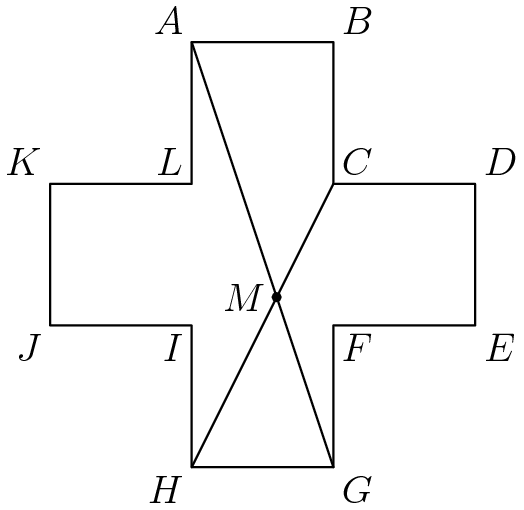
\includegraphics[height=8cm,page=1]{2021-07-31-figure-02}
\end{center}

\nopagebreak

\fbox{(A) $\dfrac{44}{3}$ \quad (B) $16$ \quad (C) $\dfrac{88}{5}$ \quad (D) $20$ \quad (E) $\dfrac{62}{3}$}

\begin{answer}
We can obtain the solution by calculating the area of rectangle $ABGH$ minus the combined area of triangles $\triangle AHG$ and $\triangle CGM$.

We know that triangles $\triangle AMH$ and $\triangle GMC$ are similar because $\overline{AH} \parallel \overline{CG}$. Also, since $\frac{AH}{CG} = \frac{3}{2}$, the ratio of the distance from $M$ to $\overline{AH}$ to the distance from $M$ to $\overline{CG}$ is also $\frac{3}{2}$. Solving with the fact that the distance from $\overline{AH}$ to $\overline{CG}$ is 4, we see that the distance from $M$ to $\overline{CG}$ is $\frac{8}{5}$.

The area of $\triangle AHG$ is simply $\frac{1}{2} \cdot 4 \cdot 12 = 24$, the area of $\triangle CGM$ is $\frac{1}{2} \cdot \frac{8}{5} \cdot 8 = \frac{32}{5}$, and the area of rectangle $ABGH$ is $4 \cdot 12 = 48$.

Taking the area of rectangle $ABGH$ and subtracting the combined area of $\triangle AHG$ and $\triangle CGM$ yields
\begin{align*}
48 - \left(24 + \frac{32}{5}\right) 
  = \frac{88}{5}
\end{align*}
\begin{empheq}[box={\mathbox[colback=white]}]{equation*}
    [ABCM] = \frac{88}{5}
\end{empheq} 
\end{answer}
%%%%%%%%%%%%%%%%%%%%%%%%%%%%%%%%%%%%%%%%%%%%%%%%%%%%%%%%%%%%%%%%%%%%%%%%

\iftoggle{showAnswers}{\newpage}

%%%%%%%%%%%%%%%%%%%%%%%%%%%%%%%%%%%%%%%%%%%%%%%%%%%%%%%%%%%%%%%%%%%%%%%%
\subsection*{3.}

\nopagebreak

A paint brush is swept along both diagonals of a square to produce the symmetric painted area, as shown. Half the area of the square is painted. What is the ratio of the side length of the square to the brush width?

\nopagebreak

\begin{center}
  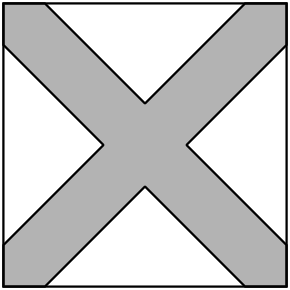
\includegraphics[height=5cm,page=1]{2021-07-31-figure-03}
\end{center}

\nopagebreak

\fbox{(A) $2\sqrt{2}+1$ \quad (B) $3\sqrt{2}$ \quad (C) $2\sqrt{2}+2$ \quad (D) $3\sqrt{2}+1$ \quad (E) $3\sqrt{2}+2$}

\begin{answer}
Let $w$ be the width of the brush. Without loss of generality, let the side length of the square be $1$ unit. 
\bigskip
\begin{center}
  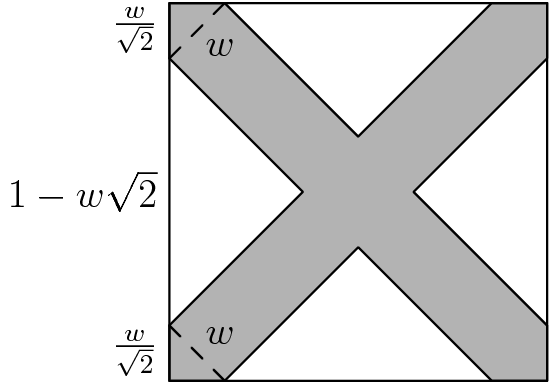
\includegraphics[height=5cm,page=1]{2021-07-31-figure-03b}
\end{center}
\bigskip
The painted area cuts off two segments of length $w/\sqrt{2}$, leaving a segment of length
\begin{align*}
1 - 2 \cdot \frac{w}{\sqrt{2}} = 1 - w \sqrt{2}
\end{align*}
This length is the hypotenuse of a $45$-$45$-$90$ unpainted triangle, so each leg has length
\begin{align*}
\frac{1 - w \sqrt{2}}{\sqrt{2}}
\end{align*}
Then the area of each such 45-45-90 unpainted triangle is
\begin{align*}
\frac{1}{2} \left( \frac{1 - w \sqrt{2}}{\sqrt{2}} \right)^2 = \frac{(1 - w \sqrt{2})^2}{4}
\end{align*}
Hence, the total unpainted area is
\begin{align*}
4 \cdot \frac{(1 - w \sqrt{2})^2}{4} = (1 - w \sqrt{2})^2 = \frac{1}{2}
\end{align*}
Taking the square root of both sides, we get
\begin{align*}
1 - w \sqrt{2} = \frac{1}{\sqrt{2}} = \frac{\sqrt{2}}{2}
\end{align*}
so
\begin{align*}
w \sqrt{2} = 1 - \frac{\sqrt{2}}{2} = \frac{2 - \sqrt{2}}{2}
\end{align*}
Then
\begin{align*}
w = \frac{2 - \sqrt{2}}{2 \sqrt{2}} = \frac{(2 - \sqrt{2}) \sqrt{2}}{4} = \frac{2 \sqrt{2} - 2}{4} = \frac{\sqrt{2} - 1}{2}
\end{align*}
Hence, the ratio of the side length of the square to the brush width is
\begin{align*}
\frac{1}{w} 
  = \frac{2}{\sqrt{2}-1} 
  = \frac{2 (\sqrt{2}+1)}{(\sqrt{2}-1)(\sqrt{2}+1)} 
  = 2\sqrt{2} + 2
\end{align*}
\begin{empheq}[box={\mathbox[colback=white]}]{equation*}
    2\sqrt{2} + 2
\end{empheq} 
\end{answer}
%%%%%%%%%%%%%%%%%%%%%%%%%%%%%%%%%%%%%%%%%%%%%%%%%%%%%%%%%%%%%%%%%%%%%%%%

\iftoggle{showAnswers}{\newpage}

%%%%%%%%%%%%%%%%%%%%%%%%%%%%%%%%%%%%%%%%%%%%%%%%%%%%%%%%%%%%%%%%%%%%%%%%
\subsection*{4.}

\nopagebreak

A fly trapped inside a cubical box with side length 1 meter decides to relieve its boredom by visiting each corner of the box. It will begin and end in the same corner and visit each of the other corners exactly once. To get from a corner to any other corner, it will either fly or crawl in a straight line. What is the maximum possible length, in meters, of its path?

\nopagebreak

\fbox{(A) $4+4\sqrt{2}$ \quad (B) $2+4\sqrt{2}+2\sqrt{3}$ \quad (C) $2+3\sqrt{2}+3\sqrt{3}$ \quad (D) $4\sqrt{2}+4\sqrt{3}$ \quad (E) $3\sqrt{2}+5\sqrt{3}$}

\begin{answer}
The path of the fly consists of eight line segments, where each line segment goes from one corner to another corner. The distance of each such line segment is $1$, $\sqrt{2}$, or $\sqrt{3}$.

The only way to obtain a line segment of length $\sqrt{3}$ is to go from one corner of the cube to the opposite corner. Since the fly visits each corner exactly once, it cannot traverse such a line segment twice. Also, the cube has exactly four such diagonals, so the path of the fly can contain at most four segments of length $\sqrt{3}$. Hence, the length of the fly's path can be at most $4\sqrt{3}+4\sqrt{2}$. This length can be achieved by taking the path
\bigskip
\begin{center}
  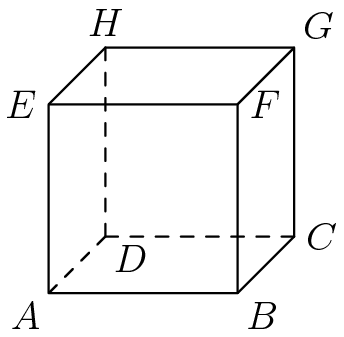
\includegraphics[height=6cm,page=1]{2021-07-31-figure-04}
\end{center}
\begin{align*}
A \rightarrow G \rightarrow B \rightarrow H \rightarrow C \rightarrow E \rightarrow D \rightarrow F \rightarrow A
\end{align*}
\begin{empheq}[box={\mathbox[colback=white]}]{equation*}
    4 \sqrt{2} + 4 \sqrt{3}
\end{empheq} 
\end{answer}
%%%%%%%%%%%%%%%%%%%%%%%%%%%%%%%%%%%%%%%%%%%%%%%%%%%%%%%%%%%%%%%%%%%%%%%%

\iftoggle{showAnswers}{\newpage}
  
%%%%%%%%%%%%%%%%%%%%%%%%%%%%%%%%%%%%%%%%%%%%%%%%%%%%%%%%%%%%%%%%%%%%%%%%
\subsection*{5.}

\nopagebreak

A cube with side length 1 is sliced by a plane that passes through two diagonally opposite vertices $A$ and $C$ and the midpoints $B$ and $D$ of two opposite edges not containing $A$ or $C$, as shown. What is the area of quadrilateral $ABCD$?

\nopagebreak

\begin{center}
  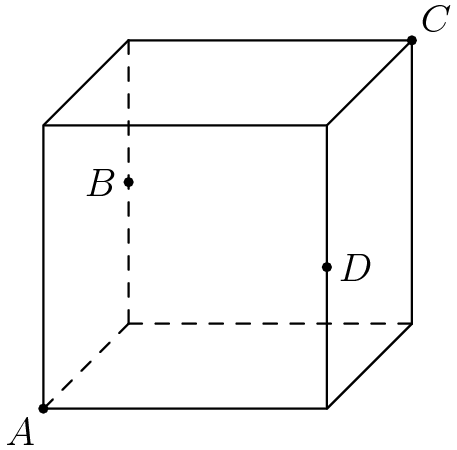
\includegraphics[height=6cm,page=1]{2021-07-31-figure-05}
\end{center}

\nopagebreak

\fbox{(A) $\dfrac{\sqrt{6}}{2}$ \quad (B) $\dfrac{5}{4}$ \quad (C) $\sqrt{2}$ \quad (D) $\dfrac{3}{2}$ \quad (E) $\sqrt{3}$}

\begin{answer}
\bigskip
\begin{center}
  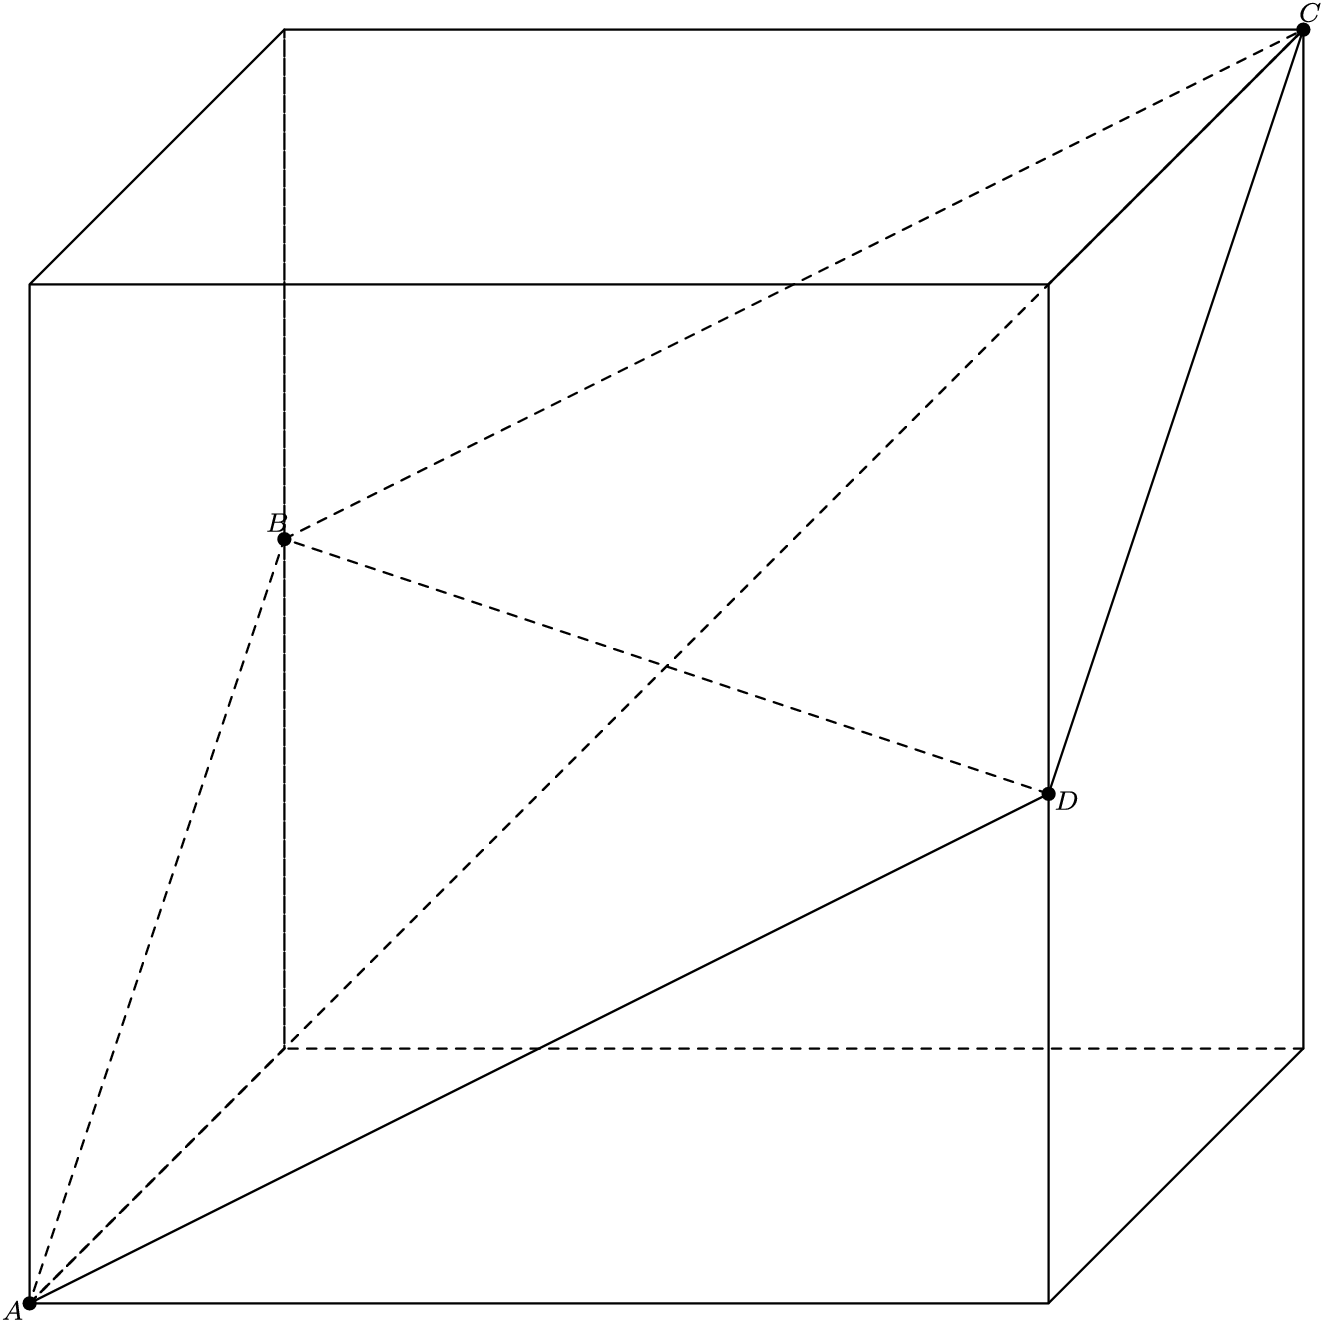
\includegraphics[width=0.4\linewidth,page=1]{2021-07-31-figure-05b}\hfill
  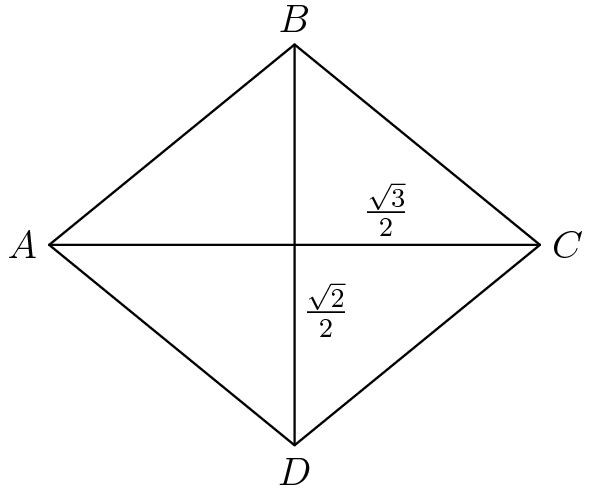
\includegraphics[width=0.4\linewidth,page=1]{2021-07-31-figure-05c}
\end{center}
\begin{align*}
AB = AD = CB = CD = \sqrt{\left(\frac{1}{2}\right)^2+1^2}
\end{align*}
it follows that $ABCD$ is a rhombus. The area of the rhombus can be computed by the formula $A = \frac 12 d_1d_2$, where $d_1,\,d_2$ are the diagonals of the rhombus (or of a kite in general). 
$BD$ has the same length as a face diagonal, or $\sqrt{1^2 + 1^2} = \sqrt{2}$. $AC$ is a space diagonal, with length $\sqrt{1^2+1^2+1^2} = \sqrt{3}$. Thus
$A = \frac 12 \times \sqrt{2} \times \sqrt{3}$ 
\begin{empheq}[box={\mathbox[colback=white]}]{equation*}
    A = \frac{\sqrt{6}}{2}
\end{empheq} 
\end{answer}
%%%%%%%%%%%%%%%%%%%%%%%%%%%%%%%%%%%%%%%%%%%%%%%%%%%%%%%%%%%%%%%%%%%%%%%%

\iftoggle{showAnswers}{\newpage}

%%%%%%%%%%%%%%%%%%%%%%%%%%%%%%%%%%%%%%%%%%%%%%%%%%%%%%%%%%%%%%%%%%%%%%%%
\subsection*{6.}

\nopagebreak

A pyramid with a square base is cut by a plane that is parallel to its base and is 2 units from the base. The surface area of the smaller pyramid that is cut from the top is half the surface area of the original pyramid. What is the altitude of the original pyramid?

\nopagebreak

\fbox{(A) $2$ \quad (B) $2+\sqrt{2}$ \quad (C) $1+2\sqrt{2}$ \quad (D) $4$ \quad (E) $4+2\sqrt{2}$}

\begin{answer}
Since the two pyramids are similar, the ratio of the altitudes is the square root of the ratio of the surface areas.
\bigskip
\begin{center}
  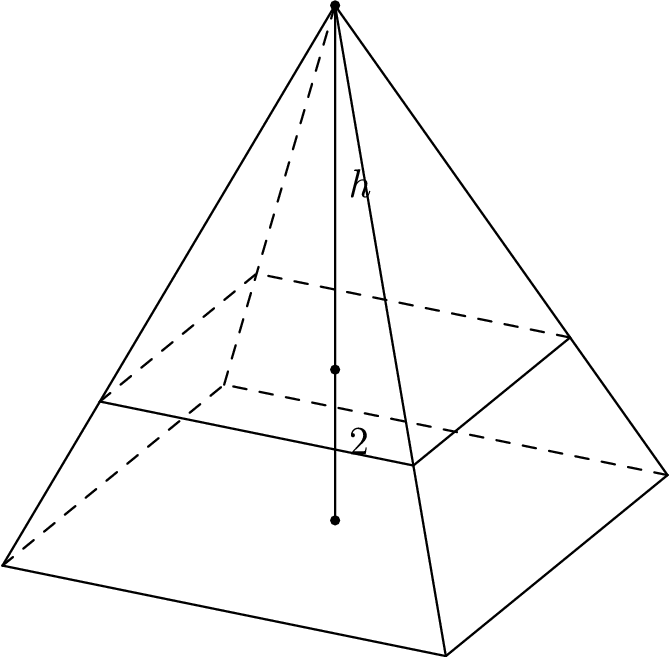
\includegraphics[height=8cm,page=1]{2021-07-31-figure-06}
\end{center}
\bigskip
If $a$ is the altitude of the larger pyramid, then $a-2$ is the altitude of the smaller pyramid.
\begin{align*}
\frac{a}{a-2} 
    = \frac{\sqrt{2}}{1}
\implies 
a & = a\sqrt{2} - 2\sqrt{2} \\
  & = \frac{2\sqrt{2}}{\sqrt{2}-1} \\
  & = \frac{2\sqrt{2}(\sqrt{2}+1)}{(\sqrt{2}-1)(\sqrt{2}+1)} \\  
  & = \frac{4+2\sqrt{2}}{2-1} \\
  & = 4 + 2\sqrt{2}
\end{align*}
\begin{empheq}[box={\mathbox[colback=white]}]{equation*}
    4 + 2\sqrt{2}
\end{empheq} 
\end{answer}
%%%%%%%%%%%%%%%%%%%%%%%%%%%%%%%%%%%%%%%%%%%%%%%%%%%%%%%%%%%%%%%%%%%%%%%%

\iftoggle{showAnswers}{\newpage}

%%%%%%%%%%%%%%%%%%%%%%%%%%%%%%%%%%%%%%%%%%%%%%%%%%%%%%%%%%%%%%%%%%%%%%%%
\subsection*{7.}

\nopagebreak

Convex quadrilateral $ABCD$ has $AB = 9$ and $CD = 12$. Diagonals $AC$ and $BD$ intersect at $E$, $AC = 14$, and triangles $AED$ and $BEC$ have equal areas. What is $AE$?

\nopagebreak

\fbox{(A) $\dfrac{9}{2}$ \quad (B) $\dfrac{50}{11}$ \quad (C) $\dfrac{21}{4}$ \quad (D) $\dfrac{17}{3}$ \quad (E) $6$}

\begin{answer}
\bigskip
\begin{center}
  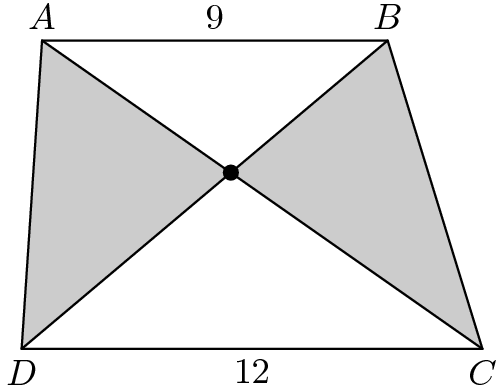
\includegraphics[height=5cm,page=1]{2021-07-31-figure-08}
\end{center}
\bigskip
Starting from equal areas:
\begin{align*}
        [AED] & = [BEC] \\
[AED] + [CDE] & = [BEC] + [CDE] \\
        [ACD] & = [BCD] 
\end{align*}
Since triangles $ACD$ and $BCD$ have the same area, they must have the same height with respect to base $CD$, and therefore $AB$ is parallel to $CD$.

Triangles $ABE$ and $CDE$ are similar, so 
\begin{align*}
\frac{AB}{CD} & = \frac{AE}{CE} \\
\frac{3}{4}   & = \frac{9}{12} \\
\implies
           AE & = \frac{3 \cdot 14}{7}
                = 6
\end{align*}
\begin{empheq}[box={\mathbox[colback=white]}]{equation*}
    6
\end{empheq} 
\end{answer}
%%%%%%%%%%%%%%%%%%%%%%%%%%%%%%%%%%%%%%%%%%%%%%%%%%%%%%%%%%%%%%%%%%%%%%%%

\iftoggle{showAnswers}{\newpage}

%%%%%%%%%%%%%%%%%%%%%%%%%%%%%%%%%%%%%%%%%%%%%%%%%%%%%%%%%%%%%%%%%%%%%%%%
\subsection*{8.}

\nopagebreak

Quadrilateral $ABCD$ has $AB = BC = CD$, $\angle ABC = 70^\circ$, and $\angle BCD = 170^\circ$. What is the degree measure of $\angle BAD$?

\nopagebreak

\fbox{(A) $75$ \quad (B) $80$ \quad (C) $85$ \quad (D) $90$ \quad (E) $95$}

\begin{answer}
Since $AB = BC$ and $\angle ABC = 70^\circ$, we have $\angle BAC = \angle BCA = (180^\circ - 70^\circ)/2 = 55^\circ$. Since $BC = CD$ and $\angle BCD = 170^\circ$, we have $\angle CBD = \angle CDB = 5^\circ$. Then $\angle ABD = \angle ABC - \angle CBD = 70^\circ - 5^\circ = 65^\circ$.

Since $\angle ABD = 65^\circ$ and $\angle BAC = 55^\circ$ are close to $60^\circ$, construct equilateral triangle $ABE$. Then $\angle DBE = \angle ABD - \angle ABE = 65^\circ - 60^\circ = 5^\circ$. But $\angle CBD = 5^\circ$, so triangles $CBD$ and $EBD$ are congruent. Hence $DE = CD$.

Since $AE = BE = DE$, $E$ is the circumcenter of triangle $ABD$. Therefore, $\angle BAD = \angle BED/2 = \angle BCD/2 = 170^\circ/2 = 85^\circ$. 
\bigskip
\begin{center}
  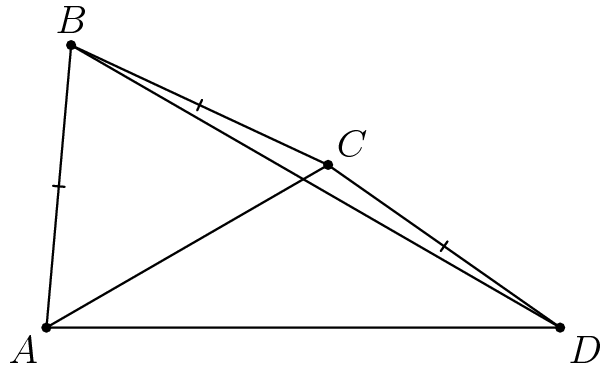
\includegraphics[width=0.3\linewidth,page=1]{2021-07-31-figure-08a}
  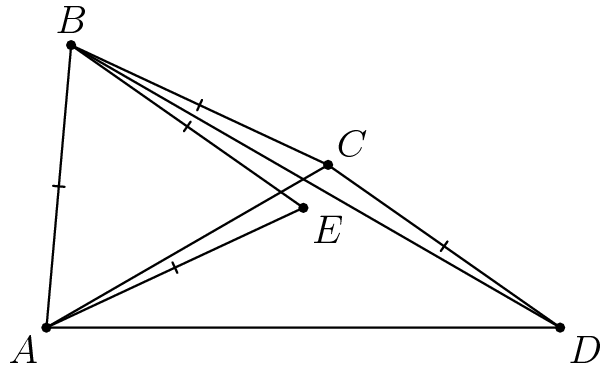
\includegraphics[width=0.3\linewidth,page=1]{2021-07-31-figure-08b}
  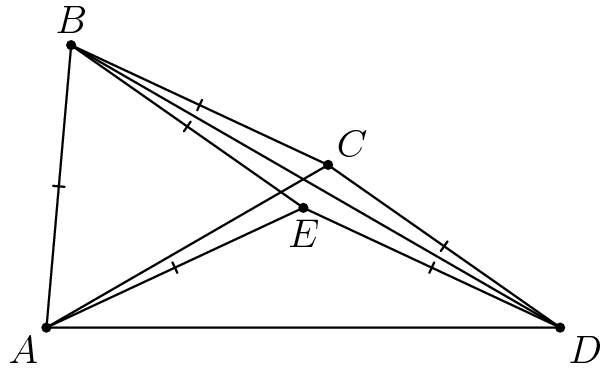
\includegraphics[width=0.3\linewidth,page=1]{2021-07-31-figure-08c}
\end{center}
\bigskip
\begin{empheq}[box={\mathbox[colback=white]}]{equation*}
    85 ~\text{degrees}
\end{empheq} 
\end{answer}
%%%%%%%%%%%%%%%%%%%%%%%%%%%%%%%%%%%%%%%%%%%%%%%%%%%%%%%%%%%%%%%%%%%%%%%%

\iftoggle{showAnswers}{\newpage}

%%%%%%%%%%%%%%%%%%%%%%%%%%%%%%%%%%%%%%%%%%%%%%%%%%%%%%%%%%%%%%%%%%%%%%%%
\subsection*{9.}

\nopagebreak

Two distinct regular tetrahedra have all their vertices among the vertices of the same unit cube. What is the volume of the region formed by the intersection of the tetrahedra?

\nopagebreak

\fbox{(A) $\dfrac{1}{12}$ \quad (B) $\dfrac{\sqrt{2}}{12}$ \quad (C) $\dfrac{\sqrt{3}}{12}$ \quad (D) $\dfrac{1}{6}$ \quad (E) $\dfrac{\sqrt{2}}{6}$}

\begin{answer}
\bigskip
\begin{center}
  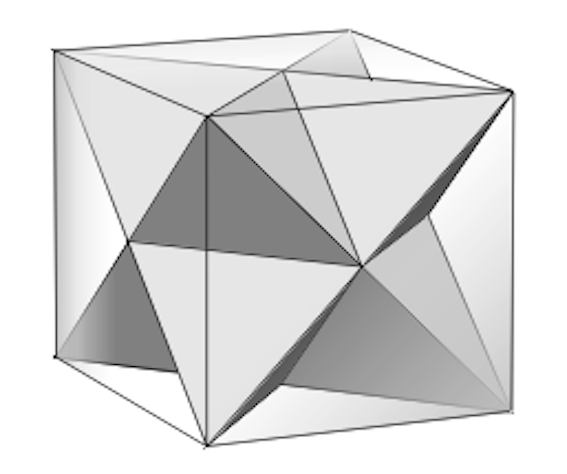
\includegraphics[height=5cm,page=1]{2021-07-31-figure-09}
\end{center}

A regular unit tetrahedron can be split into eight tetrahedra that have lengths of $1/2$. The volume of a regular tetrahedron can be found using base area and height. 

A tetrahedron of side length $1$ has base area $\dfrac{\sqrt{3}}{4}$, and height
\begin{align*}
\sqrt{1^2-\left(\frac{\sqrt{3}}{3}\right)^2}
  = \frac{\sqrt{2}}{\sqrt{3}}
 = \frac{\sqrt{2}\sqrt{3}}{3}
\end{align*}
Thus, the volume of a tetrahedron of side length $1$ is:
\begin{align*}
\frac{1}{3} \cdot \frac{\sqrt{3}}{4} \cdot \frac{\sqrt{2}\sqrt{3}}{3}
  = \frac{\sqrt{2}}{12}
\end{align*}
And a tetrahedron of side length $\sqrt{2}$ has volume
\begin{align*}
(\sqrt{2})^3  \cdot \frac{\sqrt{2}}{12}
  = \frac{1}{3}
\end{align*}

Of the eight small tetrahedra, the four tetrahedra in the corners of the large tetrahedra are not inside the other large tetrahedra. Thus, half of the large tetrahedra will not be inside of the other large tetrahedra and the intersection of the two tetrahedra is half of the previous calculation:
\begin{align*}
\frac{1}{2} \times \frac{1}{3} = \frac{1}{6}
\end{align*}
\begin{empheq}[box={\mathbox[colback=white]}]{equation*}
    \text{volume}~ = \frac{1}{6}
\end{empheq} 
\end{answer}
%%%%%%%%%%%%%%%%%%%%%%%%%%%%%%%%%%%%%%%%%%%%%%%%%%%%%%%%%%%%%%%%%%%%%%%%

\iftoggle{showAnswers}{\newpage}

%%%%%%%%%%%%%%%%%%%%%%%%%%%%%%%%%%%%%%%%%%%%%%%%%%%%%%%%%%%%%%%%%%%%%%%%
\subsection*{10.}

\nopagebreak

In trapezoid $ABCD$ with bases $AB$ and $CD$, we have $AB = 52$, $BC = 12$, $CD = 39$, and $DA = 5$. The area of $ABCD$ is

\nopagebreak

\begin{center}
  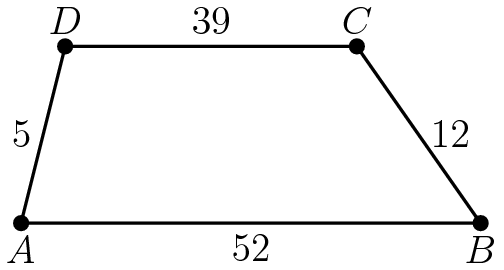
\includegraphics[height=3cm,page=1]{2021-07-31-figure-10}
\end{center}

\nopagebreak

\fbox{(A) $182$ \quad (B) $195$ \quad (C) $210$ \quad (D) $234$ \quad (E) $260$}

\begin{answer}
Extend $\overline{AD}$ and $\overline{BC}$ to meet at point $E$: 
\bigskip
\begin{center}
  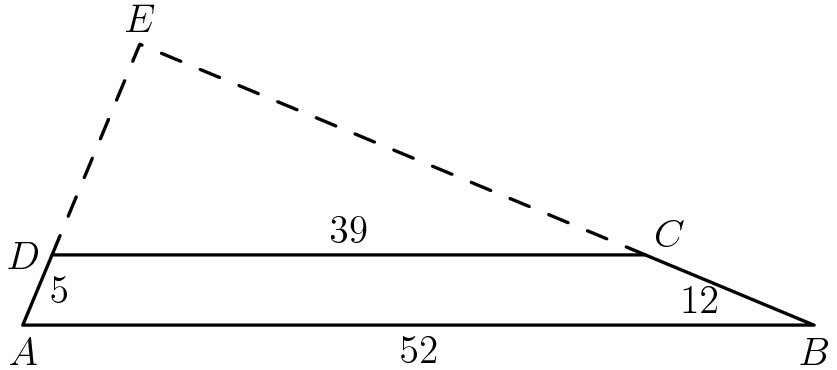
\includegraphics[height=4cm,page=1]{2021-07-31-figure-10b}
\end{center}
\bigskip
Since $\overline{AB} || \overline{CD}$ we have $\triangle AEB \sim \triangle DEC$, with ratio $\dfrac{39}{52}=\dfrac{3}{4}$. Thus 
\begin{align*} 
\frac{CE}{CE+12} = \frac{3}{4} 
  & \Longrightarrow 
  CE = 36 \\[1ex] 
\frac{DE}{DE+5} = \frac{3}{4} 
  & \Longrightarrow 
  DE = 15 
\end{align*}
So the sides of $\triangle CDE$ are $15,36,39$, which we recognize to be a $5 - 12 - 13$ right triangle. Therefore (we could simplify some of the calculation using that the ratio of areas is equal to the ratio of the sides squared),
\begin{align*}
[ABCD] 
  & = [ABE] - [CDE] \\[1ex]
  & = \frac{1}{2}\cdot 20 \cdot 48 - \frac{1}{2} \cdot 15 \cdot 36 \\[1ex]
  & = 210
\end{align*}
\begin{empheq}[box={\mathbox[colback=white]}]{equation*}
    \text{area}~ = 210
\end{empheq} 
\end{answer}
%%%%%%%%%%%%%%%%%%%%%%%%%%%%%%%%%%%%%%%%%%%%%%%%%%%%%%%%%%%%%%%%%%%%%%%%

\iftoggle{showAnswers}{\newpage}

\end{document}
